%!TEX root = thesis.tex
\chapter{Methodology}
\label{cha:method}

Empirical research by its very nature relies on quantitative information and a means of analysing this information. This chapter outlines our approach to obtaining data used to study software evolution, the {\OSYS} that were used for our analysis and the approach to selecting systems. We describe how we defined vocabulary and the method we used to extract representative vocabularies from the software systems.

\section{Data Collection} % (fold)
\label{sec:data_collection}

Quantitative research relies on the acquisition of data that is appropriate and representative of the object of study, such that this data can be analysed and interpreted to give a greater understanding of what is being studied. In this section we describe the types of data that can be used to study software evolution, our motivation for studying {\OSYS} and the systems we selected for our study.

\subsection{Types of Evolution Data} % (fold)
\label{sub:types_of_evolution_data}

Studies of software evolution rely on historical information relating to software systems. Using this information, we can construct a longitudinal representation of the software in order to analyse its evolution. This historical information falls under three classifications, as described in \cite{Vasa10a}, which are summarised in \tabref{histories}.

\begin{table*}[t]
\centering
\begin{tabular}{|p{.23\textwidth}|p{.72\textwidth}|}
\hline
{\bf History} & {\bf Description}\\
\hline \hline
Release History & Source code, binaries, release notes, and release documentation\\
\hline
Revision History & Version control logs, issue/defect records, Modification history of documentation, Wiki logs\\
\hline
Project History & Messages (email, Instant message logs), Project documentation (plans, methodology, process)\\
\hline
\end{tabular}
\vspace{0.2cm}
\caption{The different types of histories that typically provide input data for studies into software evolution}
\label{tab:histories}
\vspace{-0.2cm}
\end{table*}

\emph{Release history} is that which is composed of data that pertains to the releases of a software system. This is most commonly source code, but can also include binaries, release notes and release documentation. Studies involving the release history of software systems focus upon the outcome of changes within a software system. \emph{Revision history} on the other hand, relates to the information captured regarding change, composed of information such as version control logs, defect logs and other change documentation. Such information allows us to understand the maintenance activities of the developers involved and how it relates to change. \emph{Project history} is information relating the communication and process of those involved with the project, including email and IM logs, as well as project documentation capturing plans, methodology and process.

For our study we directly analysed the release history of the software systems, in particular, the binaries that represented individual releases. This allowed us to study the product of development efforts and gave us something concrete to analyse; it was also the most consistently available information. Furthermore, developers will aim to release only a stable build and hence an analysis of these stable releases provides an idea of the activity of the project. We augment our analysis by using \emph{revision history} and \emph{project history} as they offer an insight into the development practices.

% subsection types_of_evolution_data (end)

\subsection{Open Source Software (OSS)} % (fold)
\label{sub:open_source_software_oss_}

Open Source Software (OSS) is software that is made available under a permissive licensing scheme conforming to the Open Source Definition (OSD), as defined by the Open Source Initiative\footnote{\texttt{Open Source Initiative} \emph{http://www.opensource.org.}} that allows it to be studied, altered and re-distributed by a user for free (see \tabref{osi_criteria}). Typically, the software itself is distributed in binary form and as source code, the latter being a mandatory requirement outlined by the OSD.

\begin{table}[t]
\centering
\begin{tabular}{|p{0.21\textwidth}|p{0.74\textwidth}|}
\hline
{\bf Criteria}&{\bf Description} \\
\hline
\hline
Free \par Redistribution & Redistribution of the program, in source code or other form, must be allowed without a fee. \\
\hline
Source Code & The source code for program must be available at no charge, or a small fee to cover cost of distribution and media. Intermediate forms such as the output of a preprocessor or translator are not allowed. Deliberately obfuscated source code is not allowed. \\
\hline
Distribution of Modifications & Distribution of modified software must be allowed without discrimination, and on the same terms as the original program. \\ 
\hline
License & The license must allow modifications, derived works, be technology neutral. It must not restrict other software, and must not depend on the program being part of a particular software distribution. \\
\hline
Integrity & The license may require derived and modified works to carry a different name or version number from the original software program.  \\
\hline
No \par Discrimination & The license must not restrict the program to specific field of endeavour, and must not discriminate against any person or group of persons. \\
\hline
\end{tabular}
%\hline
\vspace{0.2cm}
\caption{The criteria that defines an Open Source Software System}
\label{tab:osi_criteria}
\end{table}

{\OSS} projects, due to their non-restrictive licensing and open philosophy, present themselves as ideal candidates for studies of software engineering. As these projects typically archive a history of their associated releases, this naturally extends to longitudinal studies, particularly that of software evolution. This is enabled by the lack of restrictions pertaining to research upon \OSYS, which allow for the analysis of systems and presentation of findings (see \emph{No Discrimination} in \tabref{osi_criteria}).

As open source projects typically encourage and are sustained by the contribution of individuals in the development community, they tend to operate in a transparent manner, making public the progress of their development efforts and subsequent releases, as well as the communication exchanges between developers involved through tools such as issue trackers and user groups. The open access to information allows an insight into the operations and practices of development teams working on non-trivial software that would not be available for a commercial software project, due to the protection of information and copyright associated with typical commercial projects.

% subsection open_source_software_oss_ (end)

\subsection{Data Acquisition} % (fold)
\label{sub:data_acquisition}

Research efforts involving quantitative analysis rely on an appropriate sampling of data. To obtain the raw data required for conducting our study, we drew upon an existing corpora of open source Java software systems known as the Helix data set \cite{Helix10a}, which was established and used as a component of the work undertaken by Vasa in \cite{Vasa10a}.

The Helix data set was composed by mining many popularly used open source project repositories. Such repositories provide a rich source of information pertaining to the studies of software, typically making available the source code and binary packages for most, if not all, of the versions that have been released as part of the project. In addition to this, most repositories provide tools such as source control, wikis and defect tracking that facilitate communication between the developers of the project and its user base.

\bigskip
The data set was composed of projects obtained from the following repositories:
\begin{enumerate}
	\item Sourceforge - {\em http://www.sourceforge.com}
	\item OW2 Consortium - {\em http://www.objectweb.org}
	\item Apache Software Foundation - {\em http://www.apache.org}
	\item Java Community Projects - {\em http://community.java.net/projects/}
	\item Google Code - {\em http://code.google.com}
	\item Eclipse Project - {\em http://www.eclipse.org}
	\item Netbeans Project - {\em http://www.netbeans.org}
\end{enumerate}

As a part of this study, we extended the Helix data set to include an up to date release history for each of the systems.

% subsection data_acquisition (end)

\subsection{Selection Criteria} % (fold)
\label{sub:selection_criteria}

To select suitable systems for our study, we leveraged a selection criteria used for studying \OSYS in the context of software evolution, as proposed by Vasa in \cite{Vasa10a}.

In their study, they define the following criteria that each project considered for selection must meet:

\begin{enumerate}
	\item The system must be developed for the Java virtual machine. Source code and compiled binaries are available for each release.
	\item The software is a single coherent system, that is, it is a distribution of a collection of related {\em components} packaged together.
	\item At least {\em 15 releases} of the system are available. Only complete releases with a version identifier are considered. Branches and releases not derived from the main system tree are ignored.  Minor and major versions are both considered (for instance, Version 2.0, 2.1 and 3.0 are all considered. In this case, the version with identifier 2.1 is often a release that provides minor enhancements and/or defect corrections).
	\item The system has been in actively development and use for at least \emph{36 months}.
	\item The system comprises of at least \emph{100 types} (\ie classes and interfaces) in all releases under study.
	\item Change logs do exist. This data provides the additional information to understand the rationale behind the changes.
\end{enumerate}

\subsubsection{Rationale of Selection Criteria} % (fold)
\label{ssub:rationale_of_selection_criteria}

The Java programming language was selected due to its popularity within the open source community as well commercial settings, which has lead to the development of a diverse range of projects spanning a variety of domains. 

Systems were required to have been in active development for at least 36 months and have no less than 15 releases to ensure that there is some level of maturity within the software systems so as to provide sufficient development history for our analysis. These exact figures were selected based on observations made by Capiluppi \cite{Capiluppi03a}, which found that only 15\% of open source projects have a development history greater than 2 years. This allowed us to focus on learning from systems that have been successful in their evolution, as opposed to those that had failed.

The requirement of having at least 100 types in any releases was imposed in order to increase the likelihood that the systems selected would be non-trivial. Further, smaller software systems limit the extent to which we can generalise due to insufficient variability. We restricted our input data to systems that provided change logs as it helped to guide our investigation by providing a supplementary explanation of abnormal behaviour throughout the course of evolution.

% subsubsection rationale_of_selection_criteria (end)

% subsection selection_criteria (end)

\subsection{Selected Systems} % (fold)
\label{sub:selected_systems}

The Helix data set comprises 50 software systems. For our study, we randomly selected a subset 34 systems with the aim of achieving an equal representation of different types of software in the Java open source community. Broadly, they fall within one of three categories: (a) Applications, (b) Frameworks, and (c) Libraries, as defined in \cite{Vasa10a}.

\emph{Applications} are software systems that are able to be executed in isolation and provide functionality that is independent of other software systems. Meanwhile, \emph{Frameworks} and \emph{Libraries} are systems that provide functionality that is designed to be extended or re-used by other software systems through an API defined by the developers. Frameworks differ from libraries in that they intend to provide an abstraction that is to be extended by those using it in order to make use of it in their systems, whereas libraries typically encapsulate functionality that is used directly within the application. As there is a fine line between whether a piece of software is considered a \emph{Framework} or a \emph{Library}, the classification was derived from the terminology used by the development team responsible for a given project.

%%% Components/Frameworks that were analyzed %%%
\begin{table*}[!]
\centering
\small
\vspace{-0.6cm}
\begin{tabular}{|l|l||c|c|r|p{0.38\textwidth}|}
\hline
{\bf Name} & {\bf Type} & {\bf Rel.} & {\bf Age} &
             {\bf Size} & {\bf Description}
\\
\hline \hline
Ant&Application&18 & 510 & 561 & Build Management System\\
\hline
Azureus&Application&52 & 348 & 3261 & BitTorrent Client\\
\hline
Checkstyle&Application&19 & 365 & 270 & Static Code Quality Checker\\
\hline
DataVision&Application&18 & 325 & 233 & Reporting tool\\
\hline
Findbugs&Application&20 & 282 & 1044 & Defect identification tool\\
\hline
Flow4J&Application&29 & 94 & 274 & Process flow modelling\\
\hline
Groovy&Application&42 & 345 & 965 & Scripting language\\
\hline
JChempaint&Application&23 & 346 & 986 & Chemistry Visualisation\\
\hline
JMeter&Application&21 & 418 & 692 & Testing tool kit\\
\hline
JabRef&Application&32 & 327 & 868 & Bibliography management\\
\hline
Jasperreports&Application&63 & 426 & 1439 & Reporting engine\\
\hline
Kolmafia&Application&102 & 265 & 662 & Role Playing Game\\
\hline
Maven&Application&15 & 225 & 437 & Build management system\\
\hline
PMD&Application&42 & 345 & 570 & Static code checker\\
\hline
Proguard&Application&24 & 417 & 561 & Java Obfuscator\\
\hline
SoapUI&Application&26 & 246 & 1400 & SOAP header monitoring tool\\
\hline
\hline
Cocoon&Framework&15 & 420 & 692 & Web application framework\\
\hline
Hibernate&Framework&60 & 438 & 1893 & Object Relational Mapping\\
\hline
Jena&Framework&25 & 452 & 915 & Semantic Web Framework\\
\hline
Spring&Framework&55 & 363 & 2593 & Lightweight J2EE framework\\
\hline
Struts&Framework&18 & 469 & 910 & Web Application Framework\\
\hline
Velocity&Framework&24 & 475 & 229 & Templating engine\\
\hline
Webwork&Framework&21 & 218 & 505 & Web App. Development\\
\hline
Wicket&Framework&39 & 295 & 803 & Web App. Development\\
\hline
XWork&Framework&26 & 288 & 304 & Generic Command Pattern\\
\hline
Freemarker&Library&17 & 390 & 287 & Template engine\\
\hline
JFreeChart&Library&21 & 377 & 587 & Charting library\\
\hline
Jung&Library&25 & 324 & 358 & Universal Graph Library\\
\hline
Log4J&Library&17 & 421 & 215 & Logging framework\\
\hline
Lucene&Library&19 & 418 & 398 & Text search engine\\
\hline
Quartz&Library&17 & 376 & 177 & Job Scheduling System\\
\hline
Saxon&Library&31 & 375 & 937 & XML and XSLT processor\\
\hline
Xalan&Library&15 & 400 & 1198 & XSLT Processor\\
\hline
Xerces&Library&20 & 496 & 710 & XML processor\\
\hline
\end{tabular}
\caption{Systems investigated - Rel. shows the total number of distinct releases analysed. Age is shown in Weeks since the first release. Size is a measure of the number of classes in the last version under analysis.}
\label{tab:systems}
%\vspace{-0.2cm}
\end{table*}

The subset of the systems that were selected from the Helix data set to use for our study (see \tabref{systems}) consists of \emph{thirty-four} systems which, altogether, account for 1011 unique releases and approximately 34,000 classes (between each of the systems and their releases).

% subsection selected_systems (end)

% section data_collection (end)

\section{Vocabulary Extraction} % (fold)
\label{sec:vocabulary_extraction}

Our study analyses the vocabulary and how it evolves over time. In this section we describe the definition of vocabulary that we used within this study and how we went about extracting a representation of vocabulary from the source code according to this definition.

\subsection{Vocabulary Definition} % (fold)
\label{ssec:vocabulary_definition}

Source code represents a substantial corpus of text that is, in most cases, entirely human-generated. Embedded within this text is semantic information regarding the problem domain that it pertains to and how the application has been built. To study the vocabulary that is used by developers, an adequate definition of what should be considered vocabulary and how it can be distinguished from other text in the source code is required.

In the following sections we outline the definitions that have been used in previous studies of source code vocabulary and provide the definition that we used in our analysis.

\subsubsection{Existing Definitions of Vocabulary} % (fold)
\label{ssub:existing_definitions_of_vocabulary}

Research in the area of source code vocabulary is currently lacking an adequate and consistent definition of vocabulary. This was noted by Delorey \etal \cite{Delorey09a}, who, given the absence of a definition, described three practical levels of abstraction at which ``word'', the atomic unit with which vocabularies are composed, could be defined at (see \tabref{word_abstraction_levels}).

\begin{table*}[t]
\centering
\begin{tabular}{|p{.21\textwidth}|p{.72\textwidth}|}
\hline
{\bf Level} & {\bf Description}\\
\hline \hline
Lexicographic & Identical strings of contiguous non-whitespace characters are considered counted as the same word \\
\hline
Syntactic & Lexicographically equivalent words are only considered equivalent if used in the same part of speech (\eg a word used in a class name that is lexicographically equivalent to a word used in a method name is not considered identical) \\
\hline
Semantic & Syntactically equivalent words are grouped only if they refer to the same definition. This requires a symbol table mapping a word to its definition.\\
\hline
\end{tabular}
\vspace{0.2cm}
\caption{The different levels of abstraction at which \emph{word} could be defined, as proposed by Delorey \etal \cite{Delorey09a}}
\label{tab:word_abstraction_levels}
\vspace{-0.2cm}
\end{table*}

From the definitions that were proposed, Delorey \etal utilised a definition of word at the \emph{syntactic} level of abstraction for their study \cite{Delorey09a}. This choice was made as they argued that words defined at the \emph{lexicographic} level of abstraction that were used frequently would also be the most polysemous\footnote{Polysemes are words that have multiple related meanings.} and homonymous\footnote{Homonyms are words that have multiple unrelated meanings.}. Furthermore, their study was limited by the lack of an adequate symbol table that could be used to take advantage of the more precise \emph{semantic} definition. In addition to the symbols used within identifiers, their study also included keywords and operators (\eg mathematical operators and scoping blocks) as part of the vocabulary, arguing that this information could contain some relevant information and hence should not be discarded.

In contrast, Abebe \etal \cite{Abebe09a}, chose to define the source code vocabulary as being the union of five vocabularies that represent different abstractions within the source code: \emph{class name vocabulary} (CV), \emph{attribute name vocabulary} (AV), \emph{function name vocabulary} (FV), \emph{parameter vocabulary} (PV), and \emph{comment vocabulary} (CoV). Their study considered the symbols used within identifiers as well as individual terms used in comments to be part of the source code vocabulary. They extrapolated individual terms from the identifiers using common naming conventions used to improve the readability of source code \cite{Reddy00a}.

% subsubsection existing_definitions_of_vocabulary (end)

\subsubsection{Defining Vocabulary} % (fold)
\label{ssub:defining_vocabulary}

In the seminal computer science textbook \emph{Structure and Interpretation of Computer Programs} \cite{Abelson96a}, Abelson and Sussman wrote the following statement regarding the responsibility of programmers when developing software: ``Programs must be written for people to read, and only incidentally for machines to execute.'' This statement is especially relevant in the context of the vocabulary used by programmers and its ability to facilitate program comprehension through the maintenance stages of evolution.

In defining vocabulary for our study, we were interested in examining the conceptual terminology that is used by developers to communicate to other developers how an application should work and how it is built; in other words, elements of the source code that developers have some control over. Accordingly, we chose to exclude keywords and operators from our vocabulary as their purpose within the code is well understood and they do not contribute anything meaningful to the semantics of individual software systems. In effect, we consider only the identifiers used by developers as being part of the vocabulary.

Our definition of vocabulary also ignores vocabulary that is only accessible within a local scope; in other words, variables that are defined within a method. This decision was made as we wanted to obtain an understanding of the use of terminology that is global within an application, and thus, be of greater importance in program comprehension. Furthermore, local variable are often named in short-hand; for instance, using the name \emph{i} instead of \emph{index} as the identifier for a variable used as an index within a for loop. These kinds of transitory variables are likely to have an undue influence on the overall vocabulary.

Overall, our definition of vocabulary includes the symbol names drawn from the identifiers from \emph{classes}, \emph{methods} (name, return type and parameter types) and \emph{fields} (name, type). This closely resembles the definition of vocabulary that was used by Abebe \etal in \cite{Abebe09a}. However, unlike their study, we do not consider the terms used within comments to be part of the vocabulary. This decision was made as we wanted to study only vocabulary that was within executable elements of the source code and because the amount and quality of commentary was likely to be inconsistent across projects. Furthermore, we combine the set of terms taken from \emph{classes}, \emph{methods} and \emph{fields} and consider a system to have a single set of vocabulary per releases. This allows us to focus our efforts on the analysis of vocabulary as a single entity, simplifying the longitudinal analysis.

% subsubsection defining_vocabulary (end)

% subsection vocabulary_definition (end)

\subsection{Extracting Vocabulary} % (fold)
\label{sub:extracting_vocabulary}

For extracting the vocabulary we used for our analysis from each of the software systems within our dataset, we utilised the \emph{Mutations} software evolution metric extraction analysis tool, which was described by Vasa in \cite{Vasa10a}. Mutations utilises the ASM bytecode analysis and manipulation framework to extract metadata associated with a Java class from its compiled binary state (.class).

\begin{table}[t]
\centering
\begin{tabular}{|l|p{0.75\textwidth}|}
	\hline
\multirow{8}{*}{\textbf{General}} & [\emph{Fully Qualified Class Name}] \\
 & Super Class Name, Interfaces Implemented \\
 & Modifiers \\ 
 & Constant Pool: Numeric, String and Type Constants\\
 & Source File Name (optional)\\
 & Enclosing Class References\\
 & Annotation*\\
 & Attribute*\\ \hline
 \textbf{Inner Class*} & Name* \\ \hline
\multirow{3}{*}{\textbf{Field*}} & Modifiers, [\emph{Name}], [\emph{Type}] \\ 
& Annotation* \\
& Attribute* \\ \hline
\multirow{4}{*}{\textbf{Method*}} & Modifiers, [\emph{Name}], [\emph{Return Type}], [\emph{Parameter Types}] \\ 
& Annotation* \\ 
& Attribute* \\ 
& Compiled Code (Java bytecode instructions) \\ \hline
\end{tabular}
\vspace{0.2cm}
\caption{Structure of a compiled Java Class. Items that end with an * indicate a cardinality of zero or more \cite{Lindholm99a}. Items enclosed within square brackets are symbol names that we mine to construct the vocabulary.}
\vspace{0.5cm}
\label{tab:class_structure}
\end{table}

Amongst the metadata collected by the tool (see \tabref{class_structure}) is information relating to the members of the class (\ie its methods and fields). This information includes, for fields, the name of the field and its type; for methods, the name of the method, its return type and the types of each of its parameters. This metadata provided the elements from which we composed the vocabulary.

In order to extract the terminology that composed the vocabulary, we extended Mutations to support the extrapolation of individual terms from these elements.

\subsubsection{Identifying Terms} % (fold)
\label{ssub:identifying_terms}

Best practices relating to naming identifiers within source code recommend using names that clearly and effectively communicate the purpose of what they represent \cite{Reddy00a}. The result of this is that developers quite often utilise identifiers that are composed of multiple words. However, for the purposes of our study we considered each word that an identifier is composed of as a separate term within the vocabulary. For instance, the identifier \emph{MainWindow} would be separated into two individual terms, \emph{main} and \emph{window}.

In order to separate compound identifiers into the individual terms that they are composed of, we required appropriate guidelines to assist us in determining when an identifier has been composed of more than one term. For our purposes, we utilised the Java Coding Style Guide \cite{Reddy00a}, which is well adhered to within the open source community, as it has style guides for developers which apply alternative casing and delimiter characters to allow easier identification of individual terms within an identifier.

For the naming of identifiers at any level of abstraction, the Java Coding Style Guide \cite{Reddy00a} prescribes the following naming styles:

\begin{description}
	\item[Pascal case] Each word begins with an uppercase letter, followed by all lowercase letters (\eg ReportWriter).
	\item[Camel case] First word begins with a lower case letter, followed by all lowercase letters. Each trailing word begins with an uppercase letter, followed by all lowercase letters (\eg writeReport).
	\item[Upper-case, underscore separated] Each word is composed of all capital letters and words are separated by an underscore (\eg REPORT\_NAME).
\end{description}

The elements of the source code that conform to these casing conventions, along with examples of terms extracted from identifiers for each casing type are highlighted in \tabref{splitting_conventions}.

\begin{table}[t]
\centering
\begin{tabular}{|p{0.18\textwidth}|p{0.25\textwidth}|p{0.25\textwidth}|p{0.22\textwidth}|}
\hline
{\bf Convention}&{\bf Element}&{\bf Identifier}&{\bf Terms} \\
\hline
\hline
Pascal case & Class names & ReportWriter & \textbf{report}, \textbf{writer} \\
\hline
Camel case & Method names, Field names (instance variables) & writeReport & \textbf{write}, \textbf{report} \\
\hline
Upper-case, underscore separated & Field names (constants) & REPORT\_NAME & \textbf{report}, \textbf{name} \\ 
\hline
\end{tabular}
%\hline
\vspace{0.2cm}
\caption{The conventions that were used to separate individual terms within compounded identifiers, along with elements that they were used for and an example of the terms produced by splitting an identifier conforming to a given convention.}
\label{tab:splitting_conventions}
\end{table}

% subsubsection identifying_terms (end)

\subsubsection{Algorithm} % (fold)
\label{sub:algorithm}

In order to extract the vocabulary from the metadata collected by Mutations, we added a module within the tool to take the relevant data that had been extracted as a result of processing each of the versions for a given system and extract the terms from each of the elements identified in the previous section. The process that is used to extract the vocabulary is outlined in \figref{vocab_metric_extraction}

The process begins by first extracting the information required to build the vocabulary from individual classes for a given release. For each class in the version being processed, we take the name of the class, as well as its set of methods and fields and extract the information required to build the vocabulary. This step consists of taking each of the elements of the different abstractions we highlighted in the previous section and isolating the identifiers within these elements. Utilising the naming conventions presented in the previous section, we separate the identifiers into individual terms. For each level of abstraction, we maintain the number of times a term has occurred.

Once the individual terms have been extracted from each of these elements, we take the term occurrence counts that were stored for class names, methods and fields and combined them into one representation of the number of times a term has been used in a class, representing the vocabulary usage for the class. While doing this, we also filter out any of the terms that were considered to be noise, as described in the next section (\subsubsecref{eliminate_noise_in_the_vocabulary}). Sample code highlighting the elements that are extracted from the code to represent the vocabulary for the class is shown in \lstref{extraction_example}. In the sample listing, the terms \emph{report}, \emph{settings}, \emph{break}, \emph{print} and \emph{writer} have been extracted and form the vocabulary for the class, while the terms \emph{get}, \emph{set} and \emph{string} have been eliminated as noise terms.

Finally, we take the vocabulary we extracted for each class and combine them together to form the vocabulary for the version as a whole, as represented by a collection of all the terms used and the number of times which they were used in the version.

\begin{figure}[t]
\centering
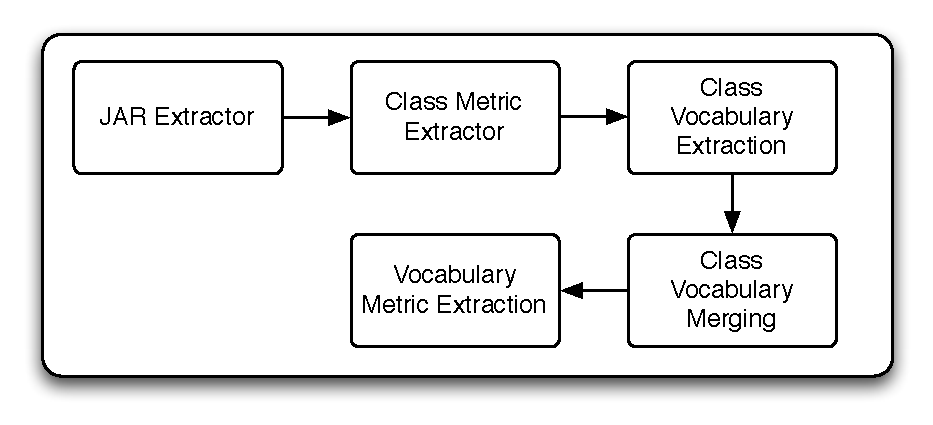
\includegraphics[width=\textwidth]{Figures/Vocab-VocabMetricExtraction.pdf}
\caption{Vocabulary metric extraction process for each release of a software system}
\label{fig:vocab_metric_extraction}
\end{figure}

\begin{lstlisting}[caption={Code sample showing the extraction of terms from various elements of the source code. Above each element is a comment describing the terms extracted from the element and the part of the element they were extracted from. At the bottom is a list of the terms extracted (including noise terms that were ignored) and their occurrence count.}, label={lst:extraction_example}, float=t]
public class ReportWriter // report, writer (class name)
{   
    // string (type); report, break (name)
    private static final String REPORT_BREAK = "----------";

    // report, settings (type); settings (name)
    private ReportSettings settings;
    
    // report, settings (return type); get, report, settings (name)
    public ReportSettings getReportSettings()
    {
        return settings;
    }
    
    // set, report, settings (name); report, settings (parameter type)
    public setReportSettings(ReportSettings settings)
    {
        this.settings = settings;
    }
    
    // print, report (name); report (parameter type)
    public void printReport(Report report)
    {
        System.out.println(REPORT_BREAK);
        
        if(settings.isTitleOutputted())
            System.out.println(report.getTitle());
            
        System.out.println(report.getBody());
        System.out.println(REPORT_BREAK);
    }

	/** Term occurrences: **/
	// - report: 9
	// - settings: 5
	// - break: 1
	// - print: 1
	// - writer: 1
	// - get: 1  (noise term -- ignored)
	// - set: 1  (noise term -- ignored)
	// - string: 1  (noise term -- ignored)
}
\end{lstlisting}

% // Class Name: ReportWriter
% // report, writer
% 
% // Constant field: String REPORT_BREAK
% // - string, report, break
% 
% // Instance variable: ReportSettings settings
% // - report, settings; settings
% 
% // Method: getReportSettings()
% // - get, report, settings (return type); report, settings (method name)
% 
% // Method: setReportSettings(ReportSettings settings)
% // - set, report, settings (method name); report, settings (method parameter type)
% 
% // Method: printReport(Report report)
% // - print, report (method name); report (method parameter type)
% 
% // Term occurrences:
% // - report: 9
% // - settings: 5
% // - break: 1
% // - print: 1
% // - writer: 1
% 
% // Noise terms eliminated:
% // - get
% // - set
% // - string

% subsubsection algorithm (end)

\subsubsection{Eliminate Noise in the Vocabulary} % (fold)
\label{ssub:eliminate_noise_in_the_vocabulary}

To allow for the extraction of vocabulary that reflected the choice of terminology utilised by the developers involved with a given project, we elected to discount terms that were overwhelmingly the most commonly used across all of the projects we analysed.

Our initial observations showed that the most frequently used terms across all of the projects we selected consisted primarily of the primitive types available within the Java language. As developers are bound by the language itself to use the types, they did not fall within our definition of vocabulary. Additionally, the frequency of their usage was sufficiently high that they were likely to deter the ability to detect changes in the rest of the vocabulary.

Amongst the most frequently used terms were those prescribed by the naming conventions to be used for writing Java code outlined in \cite{Reddy00a}. This included terms such as \emph{get} and \emph{set}, terms used for naming accessors and mutators within Java programs. As conformance to such coding styles is mandated by most successful \OSYS, these terms were also ignored.

We were able to refine our subset of vocabulary further by identifying terms that were ambiguous and not contributing any substantial meaning to the vocabulary, but were commonly found terms within each of the projects. For instance, the terms \emph{data}, \emph{name} and \emph{value} are all terms that are typically used in conjunction with other terms and on their own offer little semantic value.

Taking the notion of isolating vocabulary that was more likely to be project-specific a step further, we also compiled a list of the data structure and I/O types available within the Java SDK to be excluded from our analysis. This included extensions of primitive types (\eg BigDecimal, BigInteger), collection types (\eg ArrayList, HashMap), as well as types used for accessing data streams (\eg InputStream, OutputStream).

A complete list of the terms that were excluded from the representation of vocabulary that we analysed can be found in \appendixref{vocabulary_analysis_files}.

% subsubsection eliminate_noise_in_the_vocabulary (end)

% subsection extracting_vocabulary (end)

% section vocabulary_extraction (end)

\section{Summary} % (fold)
\label{sec:summary}

In this chapter, we described the types of historical data that can be used for studies of software evolution and the {\OSYS} that were selected for our analysis. Following this, we outlined our method for extracting vocabularies consisting of the symbol names from elements of Java source code.

The following chapter (\chapref{findings}) addresses the research questions relating to vocabulary. We describe the type of growth patterns shown by vocabulary, the manner in which vocabulary is applied in source code and the how this changes as the software evolves.

% % section summary (end)

% chapter method (end)